\documentclass{beamer}

\usepackage{graphicx}
\usepackage{caption}

\begin{document}
	
	\begin{frame}[plain]
		\begin{figure}
			\centering
			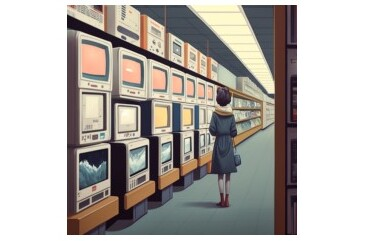
\includegraphics[width=\textwidth,height=0.85\textheight,keepaspectratio]{81.jpg}
			\caption{A long line of connected television sets stretching out along an aisle of a shop}
		\end{figure}
	\end{frame}
	
	\begin{frame}[plain]
		\begin{figure}
			\centering
			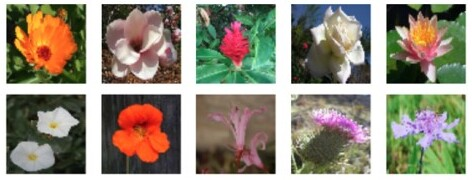
\includegraphics[width=\textwidth,height=0.85\textheight,keepaspectratio]{82.jpg}
			\caption{Example images from the Oxford 102 Flower dataset}
		\end{figure}
	\end{frame}
	
	\begin{frame}[plain]
		\begin{figure}
			\centering
			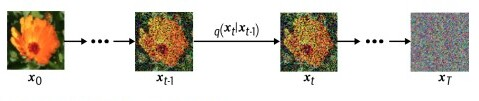
\includegraphics[width=\textwidth,height=0.85\textheight,keepaspectratio]{83.jpg}
			\caption{The forward diffusion process q}
		\end{figure}
	\end{frame}
	
	\begin{frame}[plain]
		\begin{figure}
			\centering
			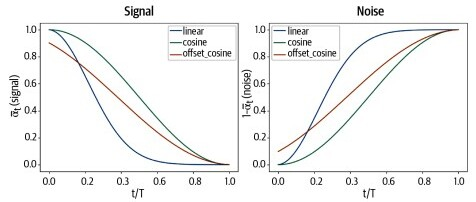
\includegraphics[width=\textwidth,height=0.85\textheight,keepaspectratio]{84.jpg}
			\caption{The signal and noise at each step of the noising process, for the linear, cosine,
				and offset cosine diffusion schedules}
		\end{figure}
	\end{frame}
	
	\begin{frame}[plain]
		\begin{figure}
			\centering
			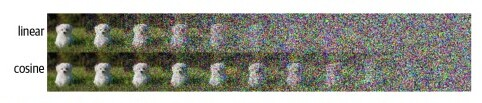
\includegraphics[width=\textwidth,height=0.85\textheight,keepaspectratio]{85.jpg}
			\caption{An image being corrupted by the linear (top) and cosine (bottom) diffusion
				schedules, at equally spaced values of t from 0 to T}
		\end{figure}
	\end{frame}
	
	\begin{frame}[plain]
		\begin{figure}
			\centering
			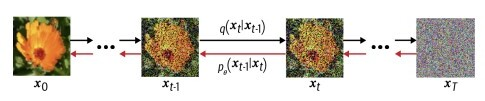
\includegraphics[width=\textwidth,height=0.85\textheight,keepaspectratio]{86.jpg}
			\caption{The reverse diffusion process $p_{\theta}(x_{t-1}\mid x_t)$ tries to undo the noise produced by the forward diffusion process.}
		\end{figure}
	\end{frame}
	
	\begin{frame}[plain]
		\begin{figure}
			\centering
			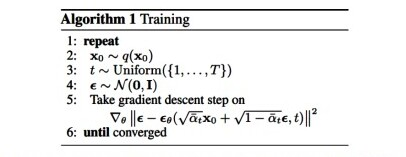
\includegraphics[width=\textwidth,height=0.85\textheight,keepaspectratio]{87.jpg}
			\caption{The training process for a denoising diffusion model}
		\end{figure}
	\end{frame}
	
	\begin{frame}[plain]
		\begin{figure}
			\centering
			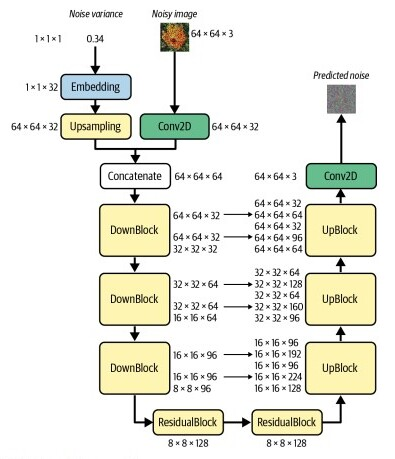
\includegraphics[width=\textwidth,height=0.85\textheight,keepaspectratio]{88.jpg}
			\caption{The training process for a denoising diffusion model}
		\end{figure}
	\end{frame}
	
	\begin{frame}[plain]
		\begin{figure}
			\centering
			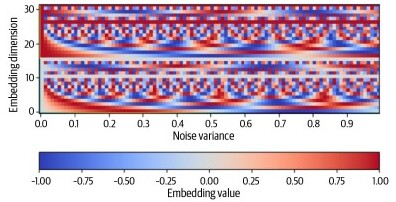
\includegraphics[width=\textwidth,height=0.85\textheight,keepaspectratio]{89.jpg}
			\caption{The pattern of sinusoidal embeddings for noise variances from 0 to 1}
		\end{figure}
	\end{frame}
	
	\begin{frame}[plain]
		\begin{figure}
			\centering
			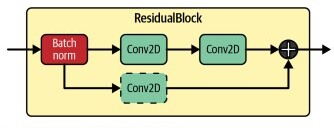
\includegraphics[width=\textwidth,height=0.85\textheight,keepaspectratio]{810.jpg}
			\caption{The ResidualBlock in the U-Net}
		\end{figure}
	\end{frame}
	
	\begin{frame}[plain]
		\begin{figure}
			\centering
			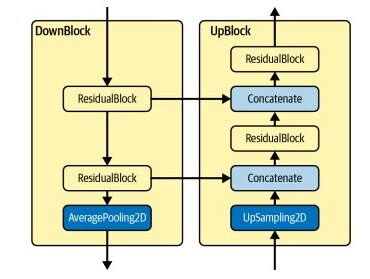
\includegraphics[width=\textwidth,height=0.85\textheight,keepaspectratio]{811.jpg}
			\caption{The DownBlock and corresponding UpBlock in the U-Net}
		\end{figure}
	\end{frame}
	
	\begin{frame}[plain]
		\begin{figure}
			\centering
			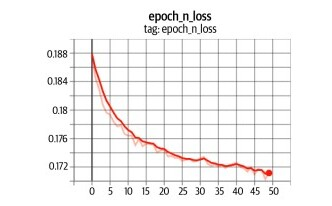
\includegraphics[width=\textwidth,height=0.85\textheight,keepaspectratio]{812.jpg}
			\caption{The noise mean absolute error loss curve, by epoch}
		\end{figure}
	\end{frame}	
	
	\begin{frame}[plain]
		\begin{figure}
			\centering
			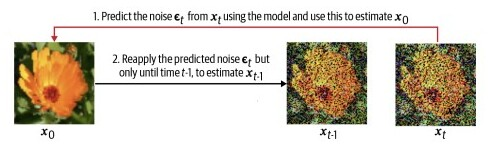
\includegraphics[width=\textwidth,height=0.85\textheight,keepaspectratio]{813.jpg}
			\caption{One step of the sampling process for our diffusion model}
		\end{figure}
	\end{frame}
	
	\begin{frame}[plain]
		\begin{figure}
			\centering
			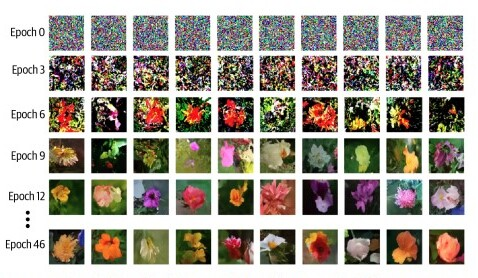
\includegraphics[width=\textwidth,height=0.85\textheight,keepaspectratio]{814.jpg}
			\caption{Samples from the diffusion model at different epochs of the training process}
		\end{figure}
	\end{frame}
	
	\begin{frame}[plain]
		\begin{figure}
			\centering
			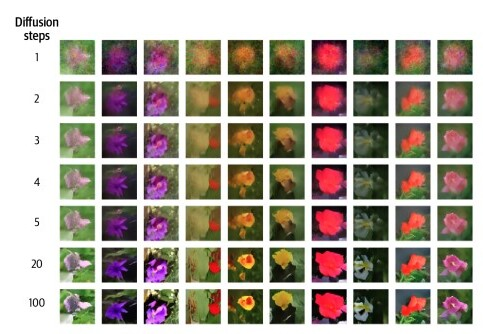
\includegraphics[width=\textwidth,height=0.85\textheight,keepaspectratio]{815.jpg}
			\caption{Image quality improves with the number of diffusion steps}
		\end{figure}
	\end{frame}
	\begin{frame}[plain]
		\begin{figure}
			\centering
			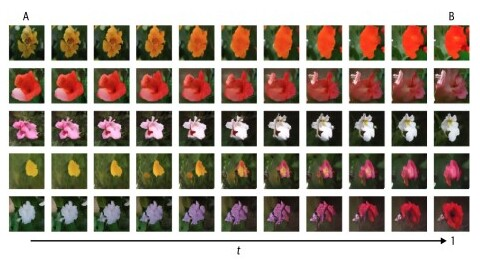
\includegraphics[width=\textwidth,height=0.85\textheight,keepaspectratio]{816.jpg}
			\caption{Interpolating between images using the denoising diffusion model}
		\end{figure}
	\end{frame}
\end{document}